86. На рисунке изображены две клетчатые фигуры: прямоугольник $7\times8$ с дыркой и буква $L$ странной формы. У каждой из фигур одна клетка отмечена чёрным. Эти фигуры по клеточкам положили на тетрадный лист так, что чёрные клетки находятся в точности друг над другом. Клетки фигуры и клетки листа совпадают. Фигурки можно поворачивать и переворачивать. Алина посчитала, сколько клеток тетрадного листа накрыто хотя бы одной из фигурок. Какие числа она могла получить? В ответ запишите {\bf все возможные} варианты через запятую.
\begin{center}
\begin{figure}[ht!]
\center{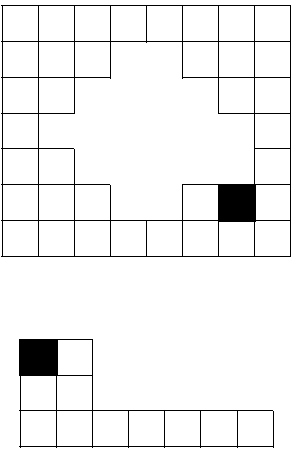
\includegraphics[scale=0.35]{15.png}}
\end{figure}
\end{center}
